%%       Generated by stratpy       %%
% remember to include \usepackage{tikz}
% and \usetikzlibrary{calc}
\begin{figure}[h]
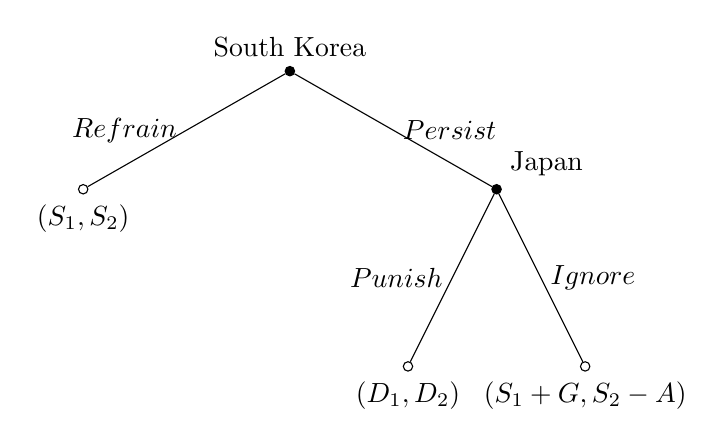
\begin{tikzpicture}[scale=1.5]

% Style for nodes
\tikzstyle{solid}=[circle,draw,inner sep=1.2,fill=black]
\tikzstyle{hollow}=[circle,draw,inner sep=1.2]
% Spacing for every level of the tree
\tikzstyle{level 1}=[level distance=10mm,sibling distance=35mm]
\tikzstyle{level 2}=[level distance=15mm,sibling distance=15mm]
% The Tree
\node(0)[solid,label=above:{South Korea}]{}child{node(1)[hollow, label=below:{$(S_1, S_2)$}]{}
    edge from parent node[left]{$Refrain$}}child{node(2)[solid, label=above right:{Japan}]{}
    child{node(3)[hollow, label=below:{$(D_1, D_2)$}]{}
    edge from parent node[left]{$Punish$}}child{node(4)[hollow, label=below:{$(S_1 + G, S_2 - A)$}]{}
    edge from parent node[right]{$Ignore$}}edge from parent node[right]{$Persist$}};
\end{tikzpicture}
\end{figure}